\documentclass{article}
\usepackage[utf8]{inputenc}
\usepackage{caption}
\usepackage{graphicx}
\usepackage{geometry}
\usepackage{subfig}
\usepackage{color}
\usepackage{natbib}
\usepackage{fancyhdr}

% Set page dimensions
\geometry{letterpaper,
total={215.9mm, 279.4mm},
left=25.4mm,
right=25.4mm,
top=25.4mm,
bottom=25.4mm}
\linespread{0.95}
\rhead{LSST Transients and Variable Stars Science Collaboration}
\begin{document}

\title{An Informal survey of Alert Broker User Requirements and Expected Capabilities}

\author{Task Force Chair: R.A. Street, Las Cumbres Observatory\\
\and
Spokesperson: Markus Rabus, PUC, Chile\\
\and
Francisco Förster Buron, CMM-UChile / MAS
\and
Suvi Gezari, University of Maryland
\and
Melissa Graham, University of Washington/LSST
\and
Ashish Mahabal, Caltech
\and
Gautham Narayan, STScI
\and
Keivan Stassun, Vanderbilt University
\and
Paula Szkody, University of Washington
\and
Stephen Smartt, Ken Smith, Queen’s University Belfast}

\maketitle

\section{Introduction}
Between February and May 2018, the Transients and Variable Stars Science Collaboration (TVS) of the Large Synoptic Survey Telescope (LSST) conducted an informal survey of science collaboration members.  The computing and software infrastructure necessary to handle LSST alerts is being developed at the time of writing, and the expectation is to use alerts from the earlier, Zwicky Transient Facility (ZTF) survey to test this infrastructure.  ZTF began commissioning in 2018, and expects to release public alerts before the end of the year.  Rather than disemminate the alerts directly ZTF expects to send the alerts to broker services, upon whom the onus is to have a public interface.  

While broker-like services have existed for many years, the majority were designed with a specific science goal, and their functionality is tailored to that goal.  In contrast, the brokers for ZTF and LSST aim to be general purpose, and expect to survey a larger community with more data.  It is therefore advantageous that they should take maximum advantage of recent software development and tools.  

The motivation behind the TVS survey was therefore to understand the scientific aims of a broker for LSST alerts as well as their practical constraints from which could be derived a set of user requirements which could be conveyed to broker developers.

Conversely, although some fields in astronomy are familiar with brokers, some are not, and each may have a different conception of what functionality to expect.  This may differ again from the functionality which is actually under development.  Therefore the survey incorporated a separate questionnaire for broker developers which aimed to provide potential users with an overview of their expected facilities.  

The questionnaire was composed using Google Forms, and distributed to the LSST Science Collaborations and community forum, with users encouraged to pass the link on to any interested parties, whether they are LSST members or not.  By the end of May 2018, 61 people had responded to the user questionnaire and 5 to the developer's questionnaire.  This report presents a summary of the results of both surveys, compiled from the Google Analytics data through the forms.  It should be noted that this questionnaire was informal (as opposed to following rigorous sociological practice) and caution should be exercised in interpreting the results.  

\subsection{Definitions}

For the purposes of the following discussion, we adopt the following definitions:

\begin{itemize}
\item Alert: A discrete package of information issued by an astronomical survey in response to the detection of a signal which is changing in brightness or position.
\item Broker: A software service that receives alerts from one or more surveys and re-distributes them, often appended with value-added information such as cross-matching the alerts with existing catalog data, or a classification of the phenomenon in question
\item Transient: An astrophysical phenomenon which does not repeat or which occurs at an unpredictable interval of time.  
\end{itemize}

\section{Broker User Requirements Survey}

For the record, the survey began with following preamble:

{\em "Survey run by the Transients and Variable Stars Science Collaboration of LSST.  

LSST is expected to produce millions of alerts every night, far exceeding the capacity of human analysts.  To maximize the science return, we need to develop software to aggregate alert and catalog data for all targets, classify them if possible and enable users to access information on candidate targets of interest to their science.

Software packages that handle these tasks are called 'brokers', and a number of them are currently being developed to serve the astronomical community.  This will be the only way to access LSST alerts.

The goals of this survey are to gain an insight into what astronomers will need from these tools, and to stimulate astronomers to consider how they will conduct their science projects in the LSST era.
 
Thank you for taking the time to help us answer these questions!   It should only take ~5-10min."}

\subsection{User Survey Respondents}
The first section of the user requirements questionnaire attempted to put the results in context by gaining an overview of what communities were represented by the respondents.  The first question inquired about the repondents areas of scientific interest, and allowed multiple answers:

\begin{enumerate}
\item {\em Please indicate the subject area(s) where you do your primary research.  Tick all that apply.}
\setcounter{enumi}{5}
\item {\em Where are you currently working?}
\item {\em Do you, your institution or the country where you are working have LSST data access rights?}
\end{enumerate}

The results are presented in Fig.~\ref{fig:Q1results}.  Transient phenomena are the most common topics of interest, but with a significant spread across subjects involving periodic targets or non-time domain science.  Moving objects are also well represented.  While efforts were made to advertize the survey outside of the LSST community, it is perhaps unsurprising that the majority of people engaged enough to answer were those who have access to LSST.  

\begin{figure}[ht]
\centering
\begin{tabular}{c}
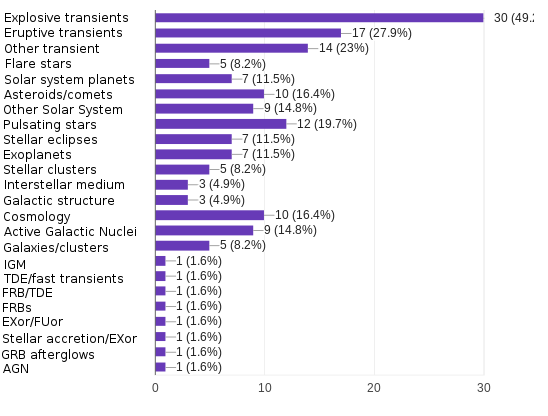
\includegraphics[width=4in]{figures/user_question_1.png}
\end{tabular}
\caption{Results of user requirements questionnaire, question 1, representing the distribution of respondent's scientific interests.  Note that multiple entries were allowed. \label{fig:Q1results}}
\end{figure}

\subsection{Alert Classification}
The classification of raw alerts according to the phenomena which caused them (as far as it can be established with the evidence available at any given time) is one of the main added-value services that current brokers provide.  Unlike most current surveys, ZTF and LSST aim to categorize all possible phenomena, including identifying the "rarest of the rare", since finding new phenomena would be one of the most exciting scientific discoveries.  But broker users must be able to extract useful information on just the subset of alerts of interest to them, implying that the search criteria will be science-specific.  The following questions attempted to gain some insight into example use-cases.  

\begin{enumerate}
\setcounter{enumi}{1}
\item {\em Target classification is another important function that brokers perform. How important is it that brokers classify your targets (as opposed to astronomers performing their own classification analysis at a later stage)? }
\item {\em Can you describe simple selection criteria for targets of interest to you that could be used to notify you if such a target is detected? For example: “notify me of all targets which have increased in brightness by $m_{\rm{SDSS-g}}$ $>$ 1 mag since the last observation and have a $(g-i)$ $>$ 1.2''}
\item {\em If Answer 3 is yes, please describe your selection criteria briefly, including all metrics of interest.}
\item {\em If Answer 3 is yes, by what mechanism would you prefer to receive alerts?  Bear in mind the alert rate could be millions per night. Check all that apply.}
\end{enumerate}

\begin{figure}[ht]
\centering
\begin{tabular}{cc}
\subfloat{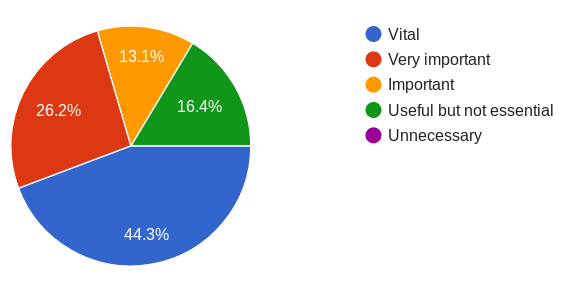
\includegraphics[width=3.2in]{figures/user_question_2.png}\label{fig:Q1results}}
\subfloat{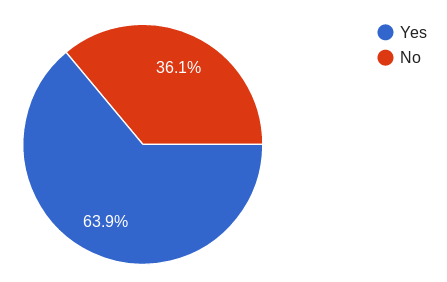
\includegraphics[width=2.5in]{figures/user_question_3.png}\label{fig:Q2results}}\\
\subfloat{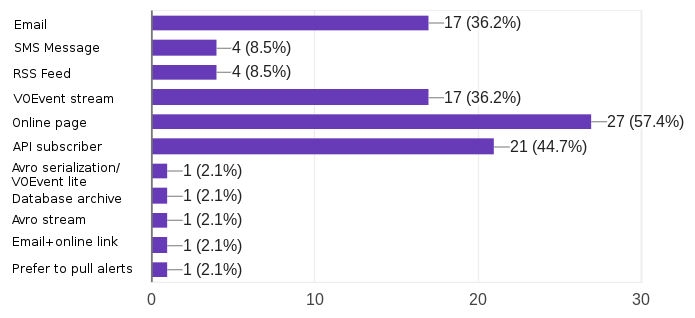
\includegraphics[width=4in]{figures/user_question_5.png}\label{fig:Q2results}}
\end{tabular}
\caption{Results of questions 2, 3 (left to right, top row) and 5 (bottom), regarding the classification functionality required from brokers. \label{fig:classification_results}}
\end{figure}

Figure~\ref{fig:classification_results} displays the results.  A large majority (83.6\%) -- though by no means all -- felt that classification was an important function for the brokers to perform.  Uses-cases of selection criteria cited included:

\begin{itemize}
\item Rise time, predicted brightness at peak, colors, photo-z of any associated galaxy magnitude threshold, amplitude of variability 
\item A known object, not a known variable, color in a specified range, brightness excursion greater than a specified tolerance
\item Notify me of all transients that, after emerging from the background, saturate in LSST colors
\item Notify me when a target is identified as significantly UNLIKE any known variable or transient
\item Notify me when an otherwise previously known regular variable star has a reported photometric measure inconsistent with that predicted by its ephemerides by > 0.5 mag.
\item Extendedness, deviation in brightness from expected brightness, change in orbital parameters
\item I'm interested in RR Lyrae stars, i.e. objects with a period between 0.2--1.0 days, that has a relatively large amplitude, $\Delta M_{\rm{SDDS-g}}$ $>$ 0.1 and in the Fourier-spectrum the main frequency has at least two harmonics with monotonically decreasing amplitudes. 
\item Unclassifiable object
\item For SNe there a few selection criteria, for example association with a host galaxy. Any physical distance information to host is extremely useful ... can calculate absolute mags. 
\item Targets which are in centers of quiescent galaxies (or within some radius of the center, still to be determined) and have not been observed there before. The color should be blue (g-r ~ -0.8 mag) and the minimum increase in brightness since the last observation > 2 mag.
\item Notify me of all targets which have increased in brightness by $m_{\rm{SDSS-g}}$ $>$ 2\,mag since the last observation, and have a $(g-r)$ $<$ 0.5.
\item All targets that have decreased in brightness by more than 5-sigma in any bandpass since the previous observation in that band. 
\item Notify me of all targets within 0.5 arcsec of an extended source that have $g-r$ $<$ 0 and have increased in brightness between the reference magnitude and the current epoch magnitude in g by more than 0.5 mag.
\item Brightness, color, ra/dec that I can check against my own catalog of interesting objects (e.g., nearby galaxies)
\item Magnitude, brightening rate, colors, position in host galaxy (center of a galaxy for selecting possible TDEs), host galaxy type, if known (starforming for core collapse supernovae), distance (for absolute magnitude estimation).
\item Notify me if solar system objects from [LIST] have been observed. Notify me if a new solar system object with [certain orbital parameters, e.g., a$>$100 AU] was discovered. 
\item Notify color evolution and rate of rise consistent with type Ia supernovae, and also light curve events that are consistent with microlensing
\item Notify me of all transients inside the LIGO spatial localization that have increased in brightness in the hour since the event criteria vary
\item Important information for follow-up observations of radio-loud AGN observed by LSST are: 1. the class of object [only radio-loud AGN]; 2. increase in brightness with respect to reference catalog(s) and with respect to previous LSST observations on different time scales (day, week, months) [increase > 1 mag]; 3. source coordinates; 4. redshift of the source [different redshift interval depending on the energy range in which the follow-up observations will be performed]
\item Object significantly brighter in u-band  
\item One example of several: is the observed brightness significantly greater than the predicted? ""predicted"" and ""significantly"" are defined from the data record in hand for that object.
\item $m(SDSS) - g$ $>$ 0.9 $g-r$ $<$ 0.7 $u-g$ $<$ 0.45
\item Brightness increase: $\geq$0.3\,mag in at least one filter for objects in star forming regions, increase u-band
\item Notify me of all targets which were undetected in all previous images (say $r$ $>$ 23) and now have (say) $r$ $<$ 20
\item For rising young/blue SNe and fast transients, $\Delta m_{\rm{SDSS-g}}$ $<$ -0.2\,mag/day and $(g-i)$ $>$ 1; for the SN cooling phase, $\Delta m_{\rm{SDSS-g}}$ $>$ 0.2\,mag/day and $(g-i)$ $<$ -0.3; for GRB afterglows $\Delta m_{\rm{SDSS-r}}$ $>$ 0.3\,mag/day and $(g-i)$ $<$ -0.4.
\item Known targets (e.g. some type of interacting binaries) that change their accretion/mass transfer rate. This can be notified as soon a change by a few magnitudes is recorded. 
\item Transients in the sense of brightening of previously unknown objects in this case to set an alert criteria is very difficult. First because often the light curve is insufficient to classify the transient and in my most recent experience even a single spectrum might not help (i.e. there is need of observing a spectral evolution). In this case I imagine one should set relatively large thresholds and perhaps match it with the with the SED of the progenitor (if available somehow). 
\item Various... e.g., solar system targets with $\Delta$ mag $>$ 0.5 relative to predicted magnitude (for given heliocentric \& geocentric distance, phase angle, and filter at time of observations); solar system targets with PSFs with FWHMs larger than 110\% of the average FWHM of nearby field stars of similar magnitude
\item Moving object brighter than predicted by $>$ 1\,mag in any band 
\item Notify me of moving targets with perihelion distance less than 1.3\,AU that have a Minimum Orbital Intersection Distance with the Earth less than 0.05\,AU and that have a delta mag greater than 0.2\,mag
\item Transient in nucleus of galaxy, no prior variability, flux increase $>$0.5\,mag, $u-g$ $<$ 0.
\item Interested in selection of high-cadence targets (DDF \& MS) based on rms variability and number of observations, e.g. $\sigma(color)$ $>$ 1\,mag and Nobs/dT $>$ 3 obs/week and dT $>$ 40 days. This can be used to build a sample of stellar rotation candidates.  Other selections of interest are cycle scale (4--10\,yr) variability, but this probably does not require an alert, rather a large selection will be done after 5 and 10 years of observations.
Quiet a few. Some of these involve distances to nearby objects, and access to historical light curves (including upper limits).
\end{itemize}

Some respondents noted the difficulty of defining a single procedure that was guaranteed to select exclusively targets of interest.  

\subsection{Geographical Distribution and Data Rights}
Researcher's interest in LSST and hence their willingness to participate in this survey may be influenced by whether they expect to have access to data from the survey.  To understand the community represented by the responses summarized here, the next questions focused on where the user currently works (since this is one of the major determinants of data access) but complemented this with a specific data rights question, to capture information on those whose membership is institutional rather than national.  The responses are represented in Figure~\ref{fig:data_access}.  
\begin{enumerate}
\setcounter{enumi}{5}
\item {\em Where are you currently working?}
\item {\em Do you, your institution or the country where you are working have LSST data access rights?}
\end{enumerate}

\begin{figure}[ht]
\centering
\begin{tabular}{cc}
\subfloat{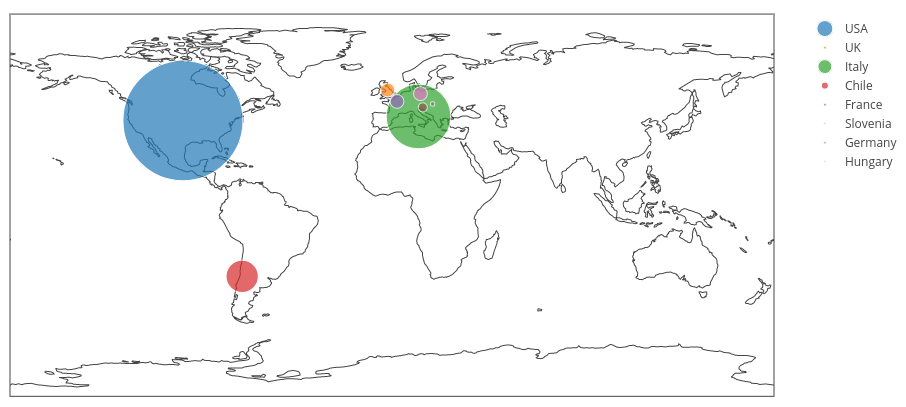
\includegraphics[width=4.5in]{figures/user_question_6_map.png}\label{fig:Q6results}}
\subfloat{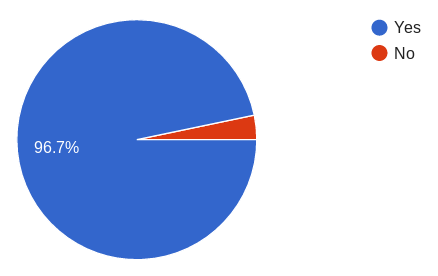
\includegraphics[width=2.0in]{figures/user_question_7.png}\label{fig:Q7results}}
\end{tabular}
\caption{Results of questions 6 \& 7 (left to right), regarding respondents current location and LSST data access rights. \label{fig:data_access}}
\end{figure}

\subsection{Alert Information Content}
The next section attempted to identify the key information users would need to receive, either in the original alert package or provided by a broker.  For the record, the questionnaire provided the following information in preamble to this section:

{\em "LSST alerts will consist of a limited package of information.  This section aims to find out if the information currently included is sufficient, and to encourage you to tell us if there are other metrics that you need.

LSST will issue one Alert for every source detected with SNR>5 in every difference image (difference = new - template; sources can be negative). A single object (supernova, variable star) would generate a new Alert every time it is detected as a source in a difference image (i.e., one Alert per detection, not one per Object). Alerts will be issued within 60 seconds of the shutter close. The Alert will contain the full record of the source that triggered the Alert (e.g., photometry, astrometry), the full record of the associated object (stationary or moving; if it exists), and the past 12 months of associated sources (i.e., previous detections at that location). These contents will also contain some variability parameters, an identifier for the nearby objects in the latest Data Release catalog, and image stamps.

For more information, see https://doi.org/10.5281/zenodo.833476 and Section 3.5.1 of the Data Products Definitions Document, linked here: https://ls.st/dpdd Tables 1, 2, and 3 document the contents of DIASource, DIAObject, and SSObject.

Please note that there is also a TVS Task Force currently reviewing which variability parameters will be calculated, which would welcome your input."} \\

The specific questions were:
\begin{enumerate}
\setcounter{enumi}{7}
\item {\em Will the information in LSST alerts be sufficient for you to identify targets of interest to your program?}
\item {\em If Answer 8 is no, what additional information would you require? Check all that apply.}
\item {\em One of a broker’s functions is to associate alerts with any catalog information that may already exist for that object.  What catalogs are (or will be) most important for your science?  Check all that apply.}
\item {\em A broker may also associate LSST alerts with those produced by other survey facilities.  What other surveys are (or will be) most important for your science? Check all that apply.}
\end{enumerate}

\begin{figure}[ht]
\centering
\begin{tabular}{c}
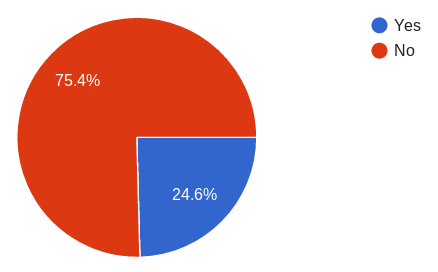
\includegraphics[width=3in]{figures/user_question_8.png}
\end{tabular}
\caption{Results of user questionnaire, questions 8, asking whether the contents of an LSST alert package will be sufficient for their scientific goals. \label{fig:Q8results}}
\label{fig:alert_content1}
\end{figure}

\begin{figure}[ht]
\centering
\begin{tabular}{c}
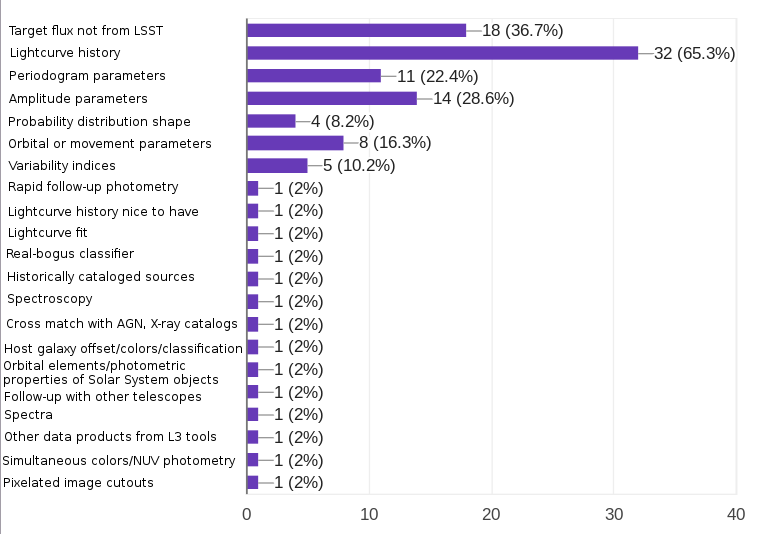
\includegraphics[width=6in]{figures/user_question_9.png}
\end{tabular}
\caption{Results of user questionnaire, questions 9, multiple choice selection of additional content that could be added to alert packets. \label{fig:Q9results}}
\label{fig:alert_content2}
\end{figure}

\begin{figure}[ht]
\centering
\begin{tabular}{c}
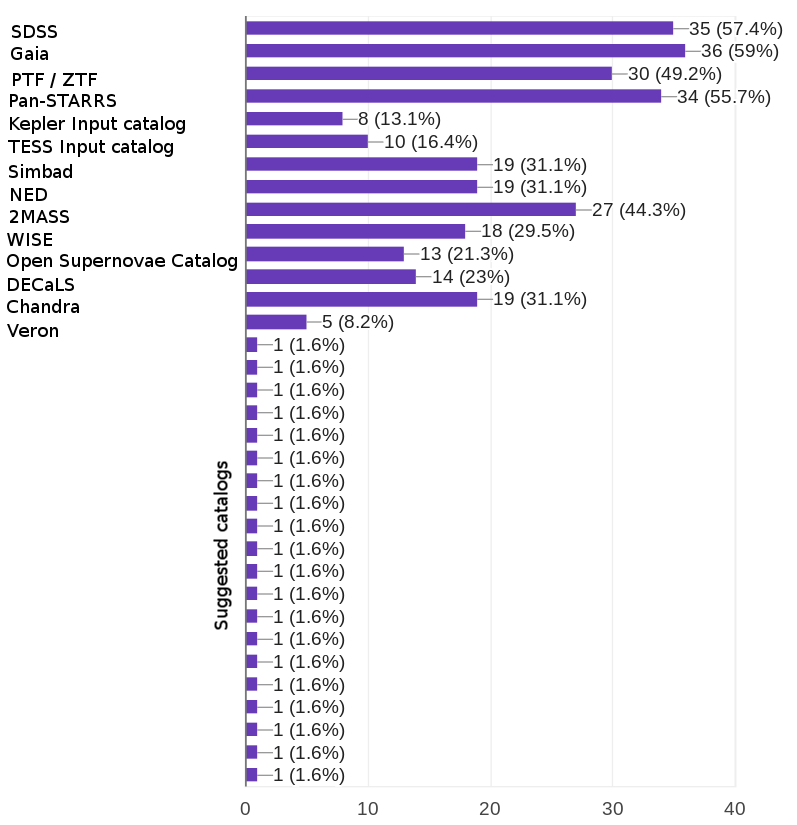
\includegraphics[width=5in]{figures/user_question_10.png}
\end{tabular}
\caption{Results of user questionnaire, questions 10, multiple choice selection of the catalogs against which alerts should be cross-matched. \label{fig:Q10results}}
\label{fig:alert_content3}
\end{figure}

\begin{figure}[ht]
\centering
\begin{tabular}{c}
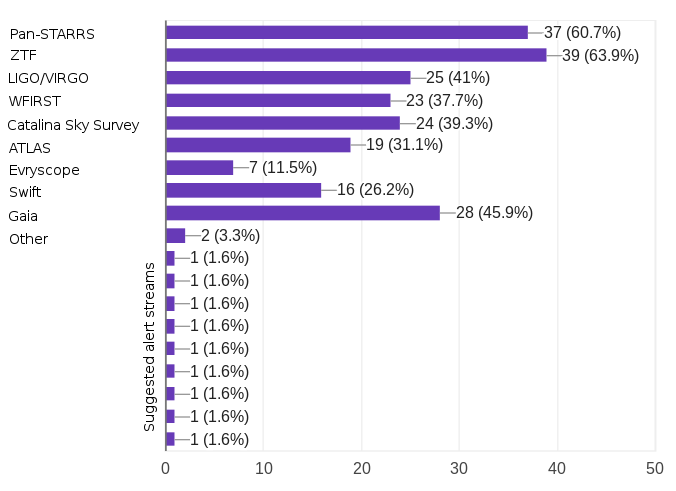
\includegraphics[width=5in]{figures/user_question_11.png}
\end{tabular}
\caption{Results of user questionnaire, questions 11, multiple choice selection of the surveys other than LSST against which alerts should be cross-matched. \label{fig:Q11results}}
\label{fig:alert_content4}
\end{figure}

Figures~\ref{fig:alert_content1} -- \ref{fig:alert_content4} indicate strongly that brokers provide a valuable service making addition data products available to users.  The lightcurve history was most frequently requested as a valuable added product, but the main goal of the question was to elicit suggestions for data products which developers may not have yet considered.  Use-cases proposed under the ``Other'' option were as follows:

\begin{itemize}
\item May need some kind of light curve fit
\item Real-bogus classifier
\item Association with historically catalogued sources at the location of the transient
\item Cross-matches with other catalogs (AGN catalogs, X-ray catalogs, etc.)
\item Host galaxy offset and colors / classification when available.
\item Followup with other telescopes to eliminate false positives
\item Spectra
\item Other data products (characterizing cometary activity levels) produced by L3 tools to be developed
\item Simultaneous color information, NUV photometry  
\item Pixelated image cutouts of the target
\end{itemize}

Question 10 invited users to consider what catalog information would be most useful to their science.  In addition to the options listed, respondents cited:

\begin{itemize}
\item VPHAS+
\item VSX
\item ``All of the above and then some: e.g. radio and gamma-ray source catalogs''
\item GCVS
\item Minor Planet Center orbital information, JPL impact hazard estimates
\item Galaxy catalog
\item Milliquas
\item PPMXL
\item GLADE catalog
\item NED-D distance catalog
\item Variable star catalogs (ASSASN, CRTS ...)
\item XMM catalogs, GALEX, photo-z catalogs, SDSS spectroscopic
\item AGN catalogs
\item DES
\item Fermi-LAT catalog
\item TeV catalog
\item SMASH
\item Minor planet center database
\item Radio catalogs: ATCA, PARKES, NVSS
\item X-ray catalogs: ROSAT, INTEGRAl, 
\item XMM-Newton
\item Swift
\item X-flux from all existing satellites, not just Chandra.
\item JPL Horizons predictions (moving objects)
\end{itemize}

Similarly, question 11 investigated which other alert sources would be valuable to cross-match against.  In addition to those listed, users highlighted:

\begin{itemize}
\item Fermi
\item ASAS-SN
\item SDSS-V
\item eROSITA
\item OGLE
\item Euclid
\item ``virtually all surveys operating on different band/color and/or different cadence should be correlated''
\end{itemize}

More than one user advocated for cross-matching against all possible alert sources, and pointed out the value of alerts coming from surveys with different observing cadences or wavelength regimes. 

\subsection{Interacting with Brokers}

The goal of the final section to the user questionnaire was to understand how user's expect to access and manipulate information from brokers.  It should be noted that these expectations may evolve with time, as scientific goals change, users become more familiar with brokers and the available technologies mature.  The following results may therefore represent a current snapshot, but offer a useful starting point for development.  The preamble of the section introduced the topic:
{\em "Astronomers may use brokers in different ways.  Some may prefer to browse targets through an interactive interface while others may prefer to develop software to interact with the broker - for example, if they need to respond rapidly to conduct follow-up observations.  These questions aim to understand how you will interact with the broker. "}

\begin{enumerate}
\setcounter{enumi}{11}
\item {\em Within what timescale do you need access to new targets of potential interest to your science, after a changing object is identified by LSST?  Recognising that individuals may have multiple science goals with different needs, tick all that apply.}
\item {\em If you interact with the broker by searching its database for targets of interest, how frequently would you expect to query it (either interactively or via software)?}
\item {\em Brokers are expected to provide online `portal' interfaces to enable users to access their information.  How do you prefer to access the information available in the brokers?   Check all that apply.}
\item {\em What essential functions would you expect from a broker’s interactive website?  Check all that apply.}
\item {\em What essential functions would you expect from a broker’s API?  Check all that apply.}
\item {\em If science-based metrics will be important for your target selection, which metrics are most essential?  Check all that apply.}
\end{enumerate}

Figure~\ref{fig:broker_interactions1} -- \ref{fig:broker_interactions6} represents the results from this section.  

\begin{figure}[ht]
\centering
\begin{tabular}{c}
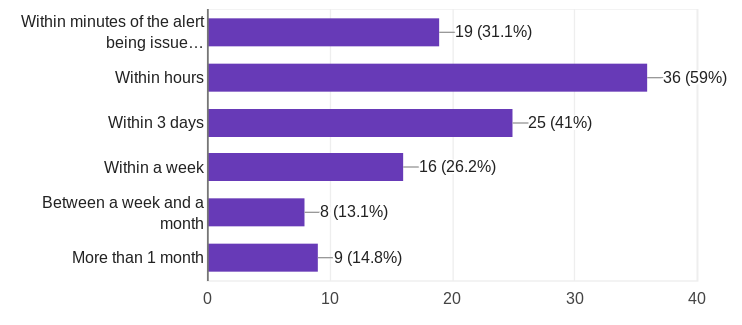
\includegraphics[width=5in]{figures/user_question_12.png}
\end{tabular}
\caption{Results of user question 12, regarding the timescale within which users need alerts to be disseminated. }
\label{fig:broker_interactions1}
\end{figure}

\begin{figure}[ht]
\centering
\begin{tabular}{c}
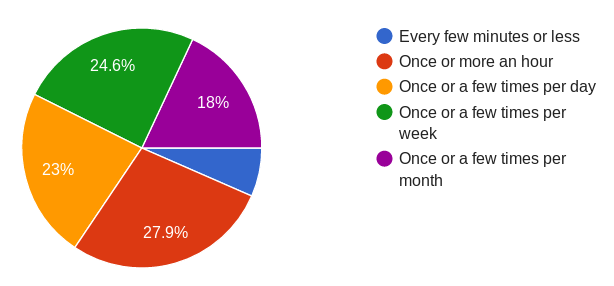
\includegraphics[width=5in]{figures/user_question_13.png}
\end{tabular}
\caption{Results of user question 13, regarding the frequency with which users expect to submit queries to a broker service. }
\label{fig:broker_interactions2}
\end{figure}

\begin{figure}[ht]
\centering
\begin{tabular}{c}
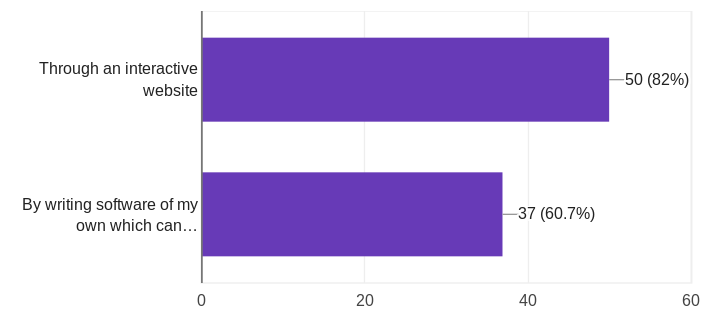
\includegraphics[width=5in]{figures/user_question_14.png}
\end{tabular}
\caption{Results of user question 14, regarding the interfaces through which users prefer to interact with the broker. }
\label{fig:broker_interactions3}
\end{figure}

\begin{figure}[ht]
\centering
\begin{tabular}{c}
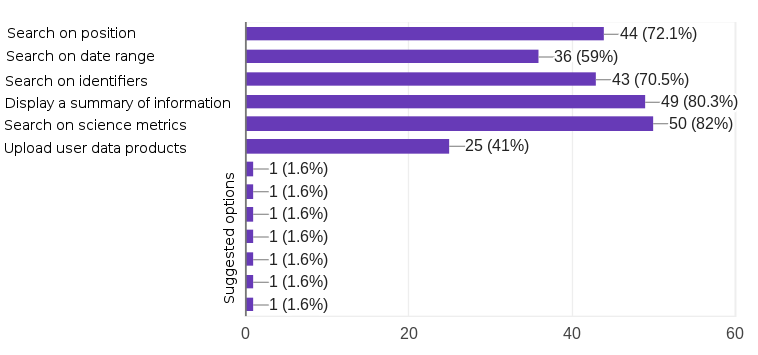
\includegraphics[width=6in]{figures/user_question_15.png}
\end{tabular}
\caption{Results of user question 15, asking what essential functions a user interface should provide.}
\label{fig:broker_interactions4}
\end{figure}

\begin{figure}[ht]
\centering
\begin{tabular}{c}
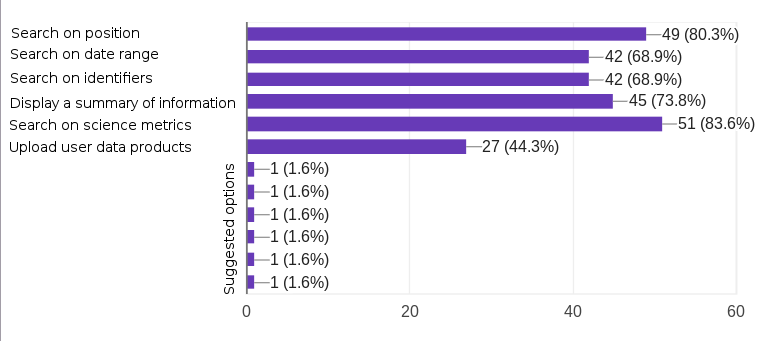
\includegraphics[width=6in]{figures/user_question_16.png}
\end{tabular}
\caption{Results of user question 16, asking what essential functions an Application Programmable Interface (API) should provide.}
\label{fig:broker_interactions5}
\end{figure}

\begin{figure}[ht]
\centering
\begin{tabular}{c}
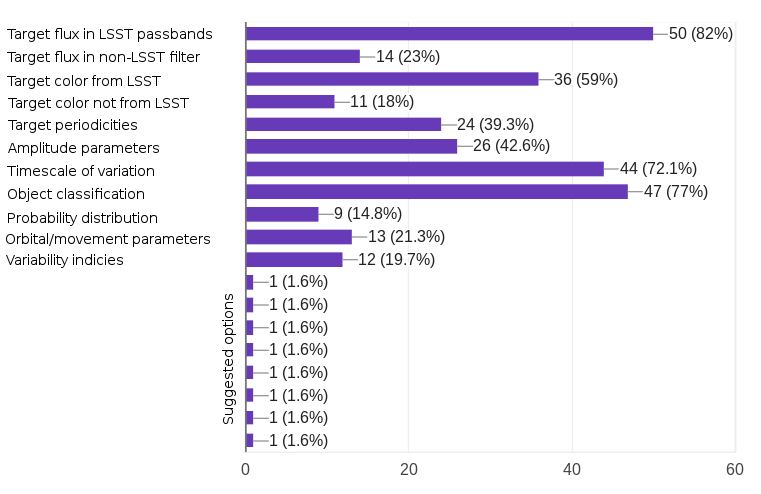
\includegraphics[width=5in]{figures/user_question_17.png}
\end{tabular}
\caption{Results of user question 17, investigating which scientific metrics or parameters will be essential search criteria when selecting targets.}
\label{fig:broker_interactions6}
\end{figure}

Users indicated a wide spread in the urgency of receiving alerts.  This could translate into changes in the broker architecture, for example if certain classifications of alerts need to be disseminated more rapidly than others.  
Figure~\ref{fig:Q13results} indicates a subset of users expect to query very frequently for alerts.  A significant fraction of users, 60.7\%, expressed the expectation of writing their own software to interact with brokers, but there is a also a clear expectation for an interactive `portal' that humans can use.  

Questions 15 and 16 asked respondents to indicate website and API functions they considered to be necessary.  In addition to the options given, they requested as follows.  

\noindent Functionality for an interactive online portal:
\begin{itemize}
\item Search by object variability class or periodicities
\item Search by new objects without prior detection
\item Search for targets by orbital parameters
\item Spectroscopic classification (needs to be feed back to broker)
\item Access to related L3 data products
\item When last observed
\item Software filters of user's own design (these could include parameters from other surveys)
\end{itemize}

\noindent API functionality:
\begin{itemize}
\item Search for potential targets based on any quantity contained in the alert packages.
\item Search by object variability class
\item Search for targets by orbital parameters
\item spectroscopic classification
\item Access to related L3 data products
\item Search on when last observed
\end{itemize}

The final question requested that users indicate the most important metrics.  In addition to those given, they requested:

\begin{itemize}
\item All available LSST measurements (all bands and epochs) on a specific target
\item Amplitude variability, after removing expected variability due to movement
\item Unclassified
\item LSST non-detections are important, cataloged source associations, distance (if associated with galaxy)
\item variability history, offset from host
\item Host galaxy offset and colors/classification, when available
\item SSObject parameters
\item ``As many of these as possible''
\end{itemize}

\section{Broker Developer's Survey}

This survey elicited five responses from representatives of development teams.  Developers were not asked to identify their specific broker, in case this discouraged responses ``on record'', so the answers give a broad overview of current development trends rather than specific insight into the state of particular projects.  Some respondents self-identified the broker they were referring to however, and are indicated in the following discussion.  

The questions posed necessarily invited more free-form text answers than in the users' survey, and began with the following preamble:
"As you know, alert broker services will be essential to fulfill the scientific potential of LSST.  Although some astronomers already use similar services, for many, LSST will be their first introduction to brokers and a number of questions are arising from the community.  We are conducting this survey of broker developers to facilitate community preparations for LSST."

The first question asked:
\begin{enumerate}
\item {\em What interfaces do you plan to use to communicate with your users?}
\end{enumerate}
{\em If you are willing/able to provide a more detailed description to (1), please enter it here}

\begin{figure}[ht]
\centering
\begin{tabular}{c}
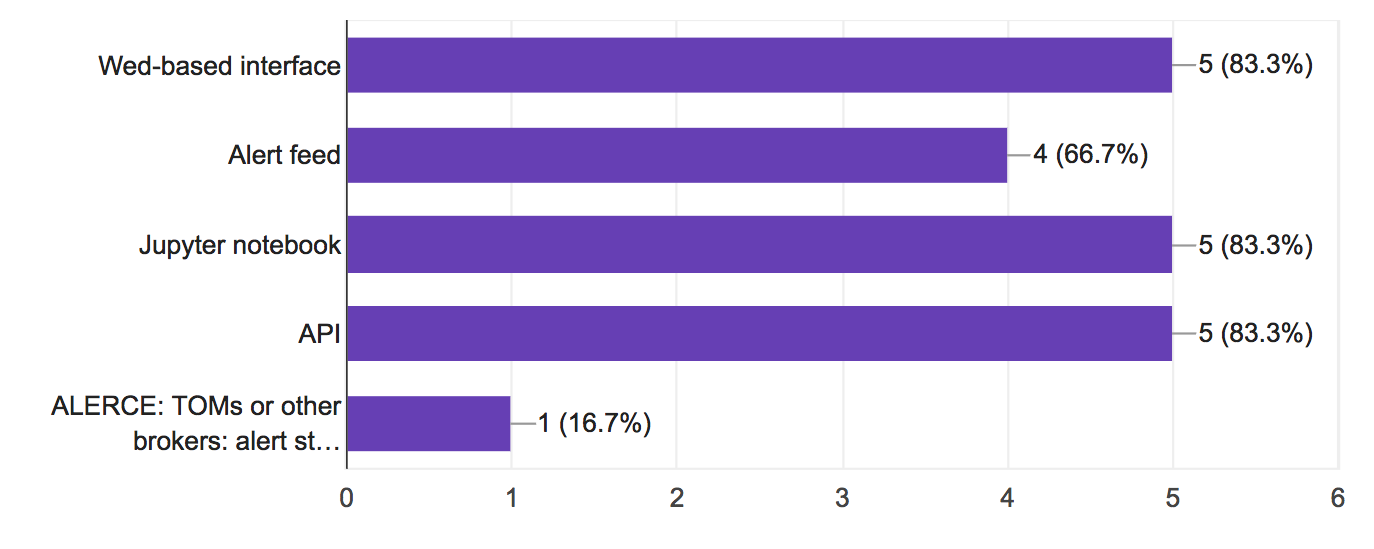
\includegraphics[width=5in]{figures/developer_question_1.png}
\end{tabular}
\caption{Results of developer question 1 regarding the user interfaces to brokers.}
\label{fig:broker_interfaces}
\end{figure}

Figure~\ref{fig:broker_interfaces} summarizes the multiple choice answers and confirms that most brokers plan to offer users a range of interfaces.  The detailed descriptions provided are given below, and attributed to a specific broker where possible. 

\begin{itemize}
\item My work is focused primarily on machine learning and backend data processing and creation, so these options would be most approachable
\item Alert stream statistics will be displayed on the web-based EPO Portal homepage and might be used within that portal as an overlay for our color image sky viewer.  EPO will store alert stream classifications from our EPO broker in our cloud-based EPO Data Center (EDC) for later querying within a Jupyter notebook or via an alert feed we expose to the public.
\item ANTARES: we are planning a few different interfaces. Web-based: Assuming this actually means browser-based, then yes, we will have pages to serve up currently active transients with high confidence of belonging to known classes + a simple search form to select objects based on most heavily used quantities in our locus-aggregated database.  Alert feed: Kafka serving Avro format alerts - same as ingest  Jupyter Notebook: limited - either our own JupyterWeb with limited storage (contingent on funding, but anticipated) or conda environment + module + template notebook that you can run yourself. The module will have a read-only interface to connect to retrieve data from our locus-aggregated database (a’la Data Lab) and will allow more complex filtering (essentially anything you care to implement within Python). We will also have a template notebook that users can use to define new “features” or stages that they want run on the LSST alert stream, but these are not guaranteed to be included, and users will have to run test data through the notebook to assess performance and utility before it will be considered.   API: We expect to have a RESTful API (GET, PUT, POST at least) that will allow the same range of queries as the python module (essentially filtering on any existing quantity within our locus-aggregated database, including position - e.g. cone searches, magnitude limits, cuts on best-guess classification).    CasJobs: Tentatively. We feel that people are moving from CasJobs to JupyterWeb, and the latter can encompass all the functionality offered by the former without people having to learn SQL, but having both may not take a very large amount of computing resources. That said, it still takes developer time, so if this gets implemented is dependent on what other feedback we get from these surveys.
\item LASAIR: Visualiation web pages for all transients, searchable database, accessible through Jupyter notebooks 
\item We plan to provide a variety of interfaces to a access combination of live data from the the event stream and historic data stored in an archive.
\item ALeRCE: The answer depends on the type of user. 1. TOMs or other brokers: alert stream 2. Astronomers: a. daily notification (includes continuous queries) b. API c. Web interface
\end{itemize}

Responses to the next question suggest that brokers do not expect any technical limitations on the number of users they could support, but the the question of data access rights remains to be fully resolved.  

\begin{enumerate}
\setcounter{enumi}{1}
\item {\em How many users will you allow? Please describe any limitations on the number of users.}
\end{enumerate}

\begin{itemize}
\item No limitations anticipated
\item Our goal is to design for 275 transactions per second but officially support 100 transactions per second.  Kafka can handle millions of writes per second on average hardware.
\item ANTARES: we don’t anticipate any practical limits for the website front end, the web API or the Kafka alert feed. For both Jupyter Hub and CasJobs, the limit on the number of users is determined by funding. Assuming this funding is fixed rather than charged to the users, and used to buy resources on a cloud platform such as AWS, the number of users is a tradeoff between the amount of disk available to each user for scratch and efficient utilization of the compute resources to process their jobs. If we allow lots of users with very little disk and our queues are filled with jobs all the time, this is not desirable, but neither is only allowing a few (~100 users) with a lot of disk, but mostly empty queues. There’s too many variables here (funding, future costs of cloud services, unknown level of demand) to provide anything more than a wild guess, but we’d like to be able to support at least 500 users on JupyterHub concurrently with access to tens of gigabytes of scratch space.
\item LASAIR: We plan to allow for very large numbers. Hundreds and we plan to build the architecture so it does not have any limitations. 
\item In theory, unlimited users. However, different groups may be limited to different quotas and have different access rights.
\item ALeRCE: To be determined
\end{itemize}

For some science use cases, rapid processing of alerts is essential.  In general, developers appear to be taking this into account and building infrastructure capable of disseminating the results as rapidly as possible.  Those that emphasize the most rapid response may reflect the expected priorites of their developers and/or national communities.  

\begin{enumerate}
\setcounter{enumi}{2}
\item {\em How fast will you process alert streams?}
\end{enumerate}

\begin{itemize}
\item Running incoming data through trained ML models should not be a major bottle neck however there are no concrete benchmarks yet 
\item Our goal is to process light curve data from the entire LSST nightly data stream every 24 hours.
\item ANTARES: The ANTARES design requirement is to process the stream in real-time -- i.e. assuming alerts are bundled by image, then $\sim$10$^{6}$ alerts every 37 seconds. We have designed the ability to throttle the feed, so if the alert rate exceeds our ability to process it, we can defer processing of an alert package from an image until periods of low-utilization. We can also select only a subset of alerts within any given alert package, focusing on sources which have a high-confidence of being astrophysical sources, rather than difference imaging artifacts or unknown moving objects.
\item LASAIR: We plan to process them as they are distributed by LSST in real time, so within minutes they should appear in the LASAIR database 
\item We are aiming to be able to process the stream at the same speed that LSST produces it.
\item ALeRCE: Our intention is to classify all alerts in less than 10 minutes. We are running simulations to assess this possibility.
\end{itemize}

Responses to question 3 indicate a preference to make brokers as access as possible, within technical limitations.  It should be noted that at the time of the questionnaire, LSST Project is in the process of drawing up more formal terms defining data access rights, which may impact the future development of brokers. 

\begin{enumerate}
\setcounter{enumi}{3}
\item {\em Will you restrict your broker to a certain community (national, scientific or otherwise)?}
\end{enumerate}

\begin{itemize}
\item No
\item No restriction (other than a bandwidth quota).  Fully open source \\(https://github.com/lsst-epo/light\_curve\_ml) and results will be stored in LSST EPO’s public cloud-based data center.
\item ANTARES: No, we consider ANTARES to be a public service. Both the JupyterHub and CasJobs systems will require user authentication, which implies some kind of registration, and it’s likely that at least initially, these will be limited to educational institutions in LSST member countries. It’s also likely that queries from a specific IP through the the RESTful API will be throttled, and users/groups that submit a large volume of queries through the API will have to register for an authentication token that is transmitted with the HTTP headers. 
\item LASAIR: We plan to have two access points - one for LSST scientists who will access valued added data that includes public data annotations (e.g. x-ray, radio, NIR cross-matches) and one with LSST data annotations (e.g. LSST deep stack, photo-z from LSST). The latter must be restricted to LSST scientists 
\item Open access, but different groups may be limited to different quotas and have different access rights.
\item ALeRCE: We will not restrict access, but we will give priority to professional scientists.
\end{itemize}

As described in depth by \cite{Najita2016}, many scientific use-cases for LSST alerts will require follow-up observations to be made of selected targets in response to alerts.  Most brokers seem to regard this as outside the responsibilities of a broker, but at least one case is planning to coordinate a contemporaneous survey.  

\begin{enumerate}
\setcounter{enumi}{4}
\item {\em Do you intend to trigger follow-up telescopes directly without human intervention?}
\end{enumerate}

\begin{itemize}
\item No
\item No, but groups may choose to implement that with our feed.
\item ANTARES: ANTARES will not directly trigger follow-up, however several members of the ANTARES team are interested in TOMS, and we will make sure the API is fully capable of interacting with TOMS, and we anticipate that our output will be used for this purpose, and are designing ANTARES accordingly. 
\item LASAIR: Partly - we will enable the 4MOST survey (called TiDES, which is primarily a UK led survey) to pick objects automatically. But the trigger doesn't move the telescope, only priorities fibres. We have no plans for automated triggers of telescopes. This does not make sense anyway if the last image taken previous to a detection is $\sim$days before.  
\item Users will be able to create their own custom output VOEvent stream to do this.
\item ALeRCE: No
\end{itemize}

\begin{enumerate}
\setcounter{enumi}{5}
\item {\em Will your broker be server-client based?}
\end{enumerate}

\begin{itemize}
\item Yes, using Kafka
\item Our broker will be server based with results stored in our public cloud-based data center and exposed via a Kafka pubsub alert feed.
\item ANTARES: Yes - all of the public interfaces we outline in 1) imply a server-client architecture. 
\item LASAIR: Yes
\item Yes
\item ALeRCE: Yes, for those subscribing to our processed alert stream. See question 1.
\end{itemize}

Responses to question 7 indicated a range of different expectations of how users would interact with different brokers, with some developers taking user queries for granted while others have a different focus. 

\begin{enumerate}
\setcounter{enumi}{6}
\item {\em Do you expect users to query your broker to select targets of interest?}
\end{enumerate}

\begin{itemize}
\item I don't know, wasn't thinking about this, wouldn't be terribly difficult to add this feature given enough resources
\item Our use case is less about targets of interest but instead querying the broker results for a sample set of a certain type of astronomy phenomena (e.g. give me 50 type IIa supernovae that occurred in the last six months).  This type of query may be from a student in a classroom using a Jupyter notebook, the website displaying an aggregated metric, or an overlay on our sky viewer highlighting recent events in the current viewable region.
\item ANTARES: Queries to select targets will be supported through the browser-based interfaces (webpages, JupyterHub, CasJobs) and this is supported through the RESTful API. Users aren’t expected to do this - we’ll have webpages for several common astrophysical classes will always be available, and users can select targets belonging to those classes without any form of query. We have no control over how alert-feed subscribers choose to filter the feed and select targets. We anticipate that external brokers will want the entire alert feed, while smaller groups might choose just a subset of the feed from pre-defined endpoints. 
\item LASAIR: Yes, of course it will the main use 
\item Yes
\item ALeRCE: Yes, through our API or web interface.
\end{itemize}

As indicated in the earlier user's survey, most astronomers will be interested in alerts of a specific subset of classifications, so the next question aimed to establish whether users would have to actively query for alerts of interest each time, or could receive notifications when new ones were issued in pre-specified categories. 

\begin{enumerate}
\setcounter{enumi}{7}
\item {\em Do you expect to notify users of alerts matching pre-defined criteria for targets of interest?}
\end{enumerate}

\begin{itemize}
\item Similar to Q7, this sounds like a problem that has off-the-shelf solutions, given that our broker is running 
\item Our pubsub model allows users to subscribe to classification categories, not specific targets.
\item ANTARES: To a limited extent. As noted in 4), some of the interfaces will require authentication. This will in turn allow us to save pre-defined criteria (positions, delta magnitude, specific color ranges etc) and in the event of alerts matching those criteria, we’d send email notifications (either for individual alerts, or in the form of a digest). We do NOT anticipate push notifications to phones or through web page notifications. The only likely source requiring notifications of this sort are GW or neutrino triggers, and these groups already have such functionality implemented.
\item LASAIR: Yes 
\item Yes
\item ALeRCE: Yes, through our API or web interface.
\end{itemize}

Question 9 asked:
\begin{enumerate}
\setcounter{enumi}{8}
\item {\em Will users need to install software on their local machines to interact with your broker?}
\end{enumerate}

Figure~\ref{fig:broker_software} summarizes the responses.  Neither ANTARES nor LASAIR developers envisioned users needing to install local software. 

\begin{figure}[ht]
\centering
\begin{tabular}{c}
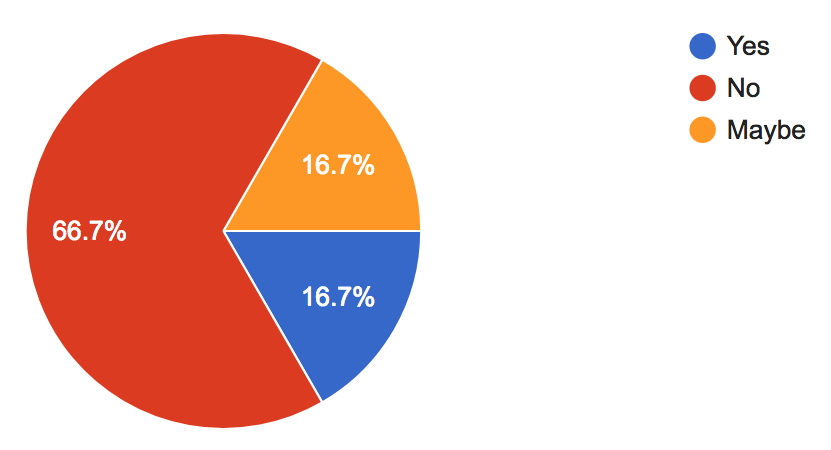
\includegraphics[width=3in]{figures/developer_question_9.png}
\end{tabular}
\caption{Results of developer question 9, asking whether users would need to install specific software on their local machine to access broker services.}
\label{fig:broker_software}
\end{figure}


\begin{enumerate}
\setcounter{enumi}{9}
\item {\em What computing resources do you expect to have or need to operate your broker? In your description, please outline any known limitations. }
\end{enumerate}

\begin{itemize}
\item AWS nodes for training ML models, hosting Kafka server, and database servers.
\item CPU/memory/database/Python – see https://github.com/lsst-epo/light\_curve\_ml   Limitations: needs light curve data with the following fields: unique identifier, labels, timestamp, magnitudes, and errors.

\item ANTARES: We currently have a modest cluster installed at NOAO for development and testing of ANTARES. \\
Each of six compute nodes has 8 cores and 32G of RAM, while the database node has 48G of RAM and 6 cores with HT.  We currently need $\sim$120T of disk (12$\times$6T SATA3 in HW RAID 6 on the database server itself), and each compute node needs $\sim$4T of local storage that is separate from the disk dedicated to the database + 1 GPU. These will be sufficient for processing ZTF in 2018, and we will add nodes and storage going forward. This should be able to handle the expected ZTF alert rate of ~1 million alerts/night with liberal filtering (assuming that real-bogus detection will not be a solved problem). Simple linear scaling is not strictly correct (particularly for disk) but we’d need $\sim$10--15 times the present level of resources for LSST. \\
We’ve begun considering how much can be accomplished using cloud-based platforms, but this is extremely challenging for real-time processing of the stream. Cloud-based solutions for some interfaces (JupyterHub/CasJobs) are tractable, and the amount of resources and limitation we’d have would be determined entirely by funding. For LSST, the anticipation is to process alerts by co-locating at NCSA in IL and running on their hardware, and while there have been discussions about this, it’s still too early to finalize this. \\
We apologize for this answer being somewhat vague, but there’s too many unconstrained variables at this juncture to be more specific, and ANTARES itself is an ongoing research project and our needs are likely to evolve before LSST.
\item LASAIR: The UK Plan is for a Data Access Centre in Edinburgh. There are proposals and plans in hand to provide the necessary infrastructure 
\item The event broker is part of the LSST:UK project to build a Data Access Centre at Edinburgh.
\item ALeRCE: It depends on the requirements.
\end{itemize}

\begin{enumerate}
\setcounter{enumi}{10}
\item {\em Does your broker have areas of preferred scientific focus? If so, what are they? }
\end{enumerate}

\begin{itemize}
\item Transient classification and anomaly detection based on light curve data
\item Education and outreach focus
\item ANTARES: With ANTARES, our focus is general purpose variable and transient classification, with an emphasis on early-classification of transients, and the identification of rare/anomalous/interesting objects (i.e. that differ to those from classes that we have trained supervised learning algorithms on).
\item LASAIR: Transients - which means not variable stars (and not low level variability of AGNS). Supernovae, kilonovae, tidal disruption events, flare stars, CVs, microlensing, AGN high amplitude variability (like TDEs and such like). 
\item The system is intended to provide support a range of different science use cases. So the core design is not aimed at any one specific area.
\item ALeRCE: At this time we are focusing on stationary objects.
\end{itemize}

\begin{enumerate}
\setcounter{enumi}{11}
\item {\em What LSST data product(s) do you expect your broker to process?}
\end{enumerate}

\begin{itemize}
\item I don't know
\item The full LSST alert stream
\item ANTARES: The LSST alert stream and periodic catalog releases. Additionally, the expectation is that LSST will make future/expected targeted pointings for images available on the same night shortly before the actual pointing is observed. This scheduling information will allow us to pre-cache sections of large databases to facilitate rapid cross-matching. 
\item LASAIR: The nightly alert steam - plus we want postage stamps of the deep stack, catalogues of LSST objects at and around the transient position, star-galaxy separation, colour of host object, and LSST photo-z. And forced photometry on the LSST data in the previous $\sim$dozen or so images stretching back $\sim$month or so 
\item The event streams from LSST and ZTF.
\item ALeRCE: From the LSST alert stream (Level 1)
\end{itemize}

\begin{enumerate}
\setcounter{enumi}{12}
\item {\em If your broker will generate an alert stream, what information will it provide?}
\end{enumerate}

\begin{itemize}
\item The classification and anomaly score of objects based on their light curves
\item Unique identifier, labels, timestamp, magnitudes, errors, and event classification
\item ANTARES: The current LSST alert package specification is not final, but ANTARES will forward the entire alert package, augmenting LSST-provided features with any that we compute from the light curve + any information on association with external catalogs + outputs of each individual classification stage, and a final “best-guess” classification and score. \\
Which stages are actually run will depend on the amount of data available for a specific alert, and potentially on the output of previous stages, so the output section of many of the stages may not be populated.  \\
We expect to maintain the Avro format. We do NOT expect to forward postage-stamp cutouts if these are embedded into the alert package by LSST (forwarding URLs to images takes considerably less bandwidth than the images themselves). 
\item LASAIR: Not yet decided. 
\item Users will be able to create their own custom output VOEvent stream.
\item ALeRCE: ID, class probabilities and uncertainties, position, time and last magnitude and error, or light curve for certain classes; known IDs in external databases. This may change depending on the community requirements.
\end{itemize}

\begin{enumerate}
\setcounter{enumi}{13}
\item {\em Will your broker classify alerts?}
\end{enumerate}

\begin{itemize}
\item Yes that is the main goal
\item Yes
\item ANTARES: Yes. We will provide probabilistic classifications as much as possible.
\item LASAIR: Yes - based on contextual information, and early lightcurve information 
\item Users will be able to select from a range of different classifiers that use different technologies to classify events.
\item ALeRCE: Yes (assign class probabilities)
\end{itemize}

It is helpful to the community to have some idea of when they can expect to begin working with new broker services, but development timelines are, as always, constrained by resources.  

\begin{enumerate}
\setcounter{enumi}{14}
\item {\em When do you expect your broker to become operational?}
\end{enumerate}

\begin{itemize}
\item I don't know
\item Currently prototyping with OGLE3 and MACHO data.  We hope to use ZTF data once it becomes available.  Fully operational when LSST alert stream goes public.
\item ANTARES: We expect an initial, feature-limited version of ANTARES to become active in Fall 2018 to process ZTF public alerts + other publicly available transient alert streams. We will be continuously building on the initial functionality and have periodic tagged releases of code.
\item LASAIR: A Version 0 is operational now at Queen's University Belfast and running in real time on Pan-STARRS and ATLAS data. LASAIR will become operational on LSST data in 2020
\item We plan to have the initial service available in time to process the LSST event stream when it becomes available. 
\item ALeRCE: Yes. The broker will be operational to incrementally larger projects until LSST starts.
\end{itemize}

\begin{enumerate}
\setcounter{enumi}{15}
\item {\em Is your broker intended to interact with other brokers?}
\end{enumerate}

\begin{itemize}
\item The incoming light curve data will be coming from other brokers I think. 
\item Potentially a Zooniverse citizen science broker
\item ANTARES: At some level all brokers are, since the LSST alert system is itself a broker. If there are other information brokers developed for LSST that prove useful (e.g. a photo-z broker, or a likely asteroid/solar system object broker) then we will try and interface with them. We also anticipate other downstream brokers will interact with ANTARES, so will make sure our API is well-documented to facilitate this. 
\item LASAIR: Yes, we can and will interact with others. This is probably straightforward. 
\item Unknown
\item ALeRCE: Yes
\end{itemize}

Figure~\ref{fig:alert_streams} summarizes the responses to question 18. 

\begin{enumerate}
\setcounter{enumi}{16}
\item {\em Do you intend to be a primary consumer of the full LSST alert stream, bearing in mind the limited number of available streams?}
\end{enumerate}

\begin{figure}[ht]
\centering
\begin{tabular}{c}
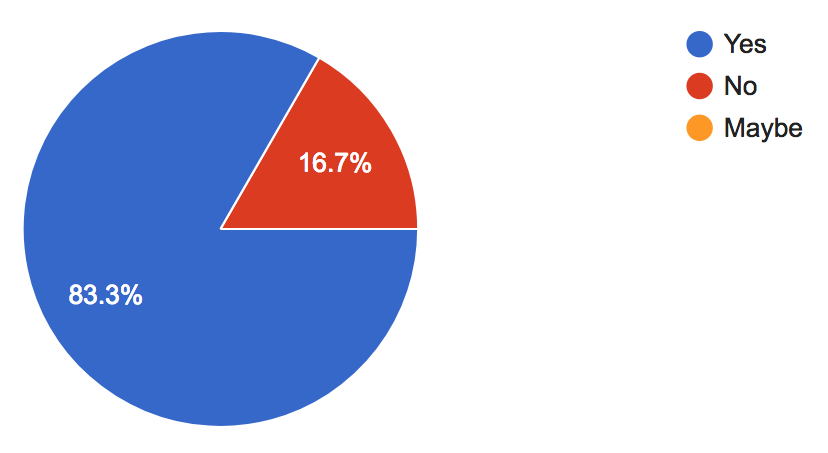
\includegraphics[width=3in]{figures/developer_question_17.png}
\end{tabular}
\caption{Results of developer question 17, asking whether a broker is expected to be a primary recipient of the full LSST alert stream.}
\label{fig:alert_streams}
\end{figure}

\begin{enumerate}
\setcounter{enumi}{17}
\item {\em What are the biggest technological challenges you have (or forsee) in bringing your broker concept into reality?}
\end{enumerate}

\begin{itemize}
\item Scaling up our ML models to match the full LSST alert stream throughput
\item Complexity of machine learning algorithms, unsupervised accuracy, database load, cost of compute resources
\item ANTARES: With ANTARES, we expect the critical challenges to be API development to fully handle real-time streaming data, and maintain the integrity of our database given myriad failure modes, most of which are not under our control. For example, PS1 has pushed images with incorrect WCS header information into their datastore on several occasions. This means that objects from these images all have the wrong coordinates, and are likely to be associated and classified incorrectly, and those values will all need removal and reprocessing from the database. Detecting these sorts of problems in a completely automated way at LSST scale is tremendously challenging. From our experience, developing a robust API for data bookkeeping will prove more challenging than actually developing the machine learning models to classify the data. \\
Accurate and useful early classification for transients remains an open problem, albeit one that we are actively working on. Very few machine learning algorithms deal with the concept of uncertainty in an input, yet this is something we require in an astronomical context, and related to the concept of confidence in the output. Adapting ML methods while building in some support for this is a challenge. \\
Maintaining provenance to replicate results at a later date is also a large problem that we are actively working on, and we anticipate most of our code to evolve significantly over the lifetime of LSST. \\
As with any software development project, maintaining funding (especially given an uncertain political climate) and personnel is a key challenge. In particular, retaining early-career academic personnel who are largely responsible for solving the technological challenges, while dealing with an academic environment that is antithetical to the work they are doing is a significant problem. 
\item LASAIR: Ensuring we have the dedicated computing infrastructure. And making a decision on what database architecture to use (currently we are planning MySQL, but we are very open to suggestions for better)  
\item We are all still learning and plans are still evolving. The challenge is to be flexible enough to adapt to changing requirements and technologies.
\item ALeRCE: No response
\end{itemize}

\begin{enumerate}
\setcounter{enumi}{17}
\item {\em What are the roadblocks to science from a broker-developer perspective?}
\end{enumerate}

\begin{itemize}
\item We require more labeled data, both classifications and labeled anomalies
\item See answer 18 above
\item ANTARES: There are many unknowns about the input alert stream at present, and broker performance for variable and transient classification will depend very strongly on real-bogus characterization and effective detection of moving objects. \\
We expect that brokers will also prove to have a significant learning curve for many users, and while we can make example notebooks and documentation, this is unquestionably a large change for the community to adapt to.  While not directly connected to brokers, effective TOMS will be critical for many science cases that brokers address, and in that respect, both efforts are strongly linked. 
\item LASAIR: Getting the funding within the UK to continue employment of key personnel. Without this, we can't deliver. 
\item Early days. We are still learning what tools will be needed. As we learn more, we will be able to develop better tools, which in turn will enable more science.
\item ALeRCE: No response
\end{itemize}

\section{}
\label{sec:references}
\bibliographystyle{plainnat}  % needs package natbib
\bibliography{references}

\end{document}
